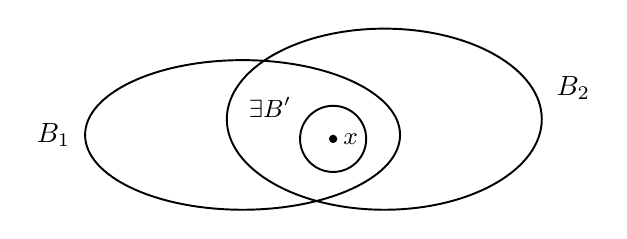
\begin{tikzpicture}[line width=0.7pt]
\draw (0,0) ellipse (2 and 0.95);
\draw (1.8,0.2) ellipse (2 and 1.15);
\node at (-2.4,0) {$B_1$};
\node at (4.2,0.6) {$B_2$};
\draw (1.15,-0.05) circle (0.42);
\fill (1.15,-0.05) circle (1.5pt) node[right] {\small $x$};
\node at (0.35,0.35) {\small $\exists B'$};
\end{tikzpicture}
